This chapter will cover evaluation steps-to-step from the baseline to the implemented solution. The performances evaluation focus mainly on two metrics : throughput and latency. Experiments could be make thanks to \acrfull{npf} \cite{barbette_tbarbettenpf_2026}.

\begin{table}[htbp]
    \centering
    \caption{Frodo server specifications}
    \label{table:frodo-specs}
    \begin{tabular}{|c|c|}
        \hline
        OS & Ubuntu 22.04.5 LTS \\
        \hline
        Kernel & 5.15.0-177-generic \\
        \hline
        CPU & Intel(R) Xeon(R) E-2378 CPU @ 2.60GHz (16 cores) \\
        \hline
    \end{tabular}
\end{table}


\begin{table}[htbp]
    \centering
    \caption{SmartNIC speficication}
    \label{table:smartnic-specs}
        \begin{tabular}{|c|c|}
        \hline
        Model & Mellanox Connect-6 \\
        \hline
        OS & Ubuntu 22.04.5 LTS \\
        \hline
        Kernel & 5.15.0-1082-bluefield \\
        \hline
        CPU & ARM Cortex-A72 (8 cores) \\
        \hline
    \end{tabular}
\end{table}

\section{Disk performances baseline}

The first step in the measurements process is to evaluate the \acrfull{io} baseline performances of the disk, with and without \acrshort{spdk}. We used \texttt{\acrfull{fio}} \cite{noauthor_kernelgitaxboefiogit_nodate} with \texttt{libaio} \cite{libaio} engine to test the throughput of the Linux kernel. Then we'll use \texttt{\acrshort{spdk}} own \acrshort{bdev} \acrfull{aio} engine.

\subsection{Throughput}

% TODO : give specs of disk somewhere
% TODO : mention data availability on the repository
% INFO about disks : SQ : 64 bytes, CQ : 16 bytes, queue depth : 64, nr_request : 1023

Throughput has been evaluated for different file size, block size and \acrshort{io} depth. \acrshort{io} \acrshort{qd} is set to 1, 16 or 32 and aggregated on mean.
File size is set to 4MB, 10MB, 100MB and 1GB. 


\subsubsection{Sequential read}

Figure \ref{fig:read-bandwidth-4M} depict the throughput over 4 kilobytes and 4 megabytes block size.  Strictly speaking of maximum throughput, \acrshort{spdk} sequential read only outperforms Linux kernel by $\approx 1.282$ with respectively 7.11 GB/s \textit{versus} 7.02 GB/s. The most significant improvement are for 4 megabytes and 10 megabytes block size where \acrshort{spdk} doubles the throughput of Linux kernel. For 4MB block size, \acrshort{spdk} mean sequential read throughput is 2.1 GB/s while Linux kernel is 1.3 GB/s. For 10MB block size, \acrshort{spdk} mean sequential read throughput is 5.59 GB/s while Linux kernel is 2.76 GB/s. Figure \ref{fig:read-bandwidth-4K} follows the same trend, although there is more variability in the results.

\begin{figure}[htbp]
    \centering
    \begin{minipage}{0.48\columnwidth}
        \centering
        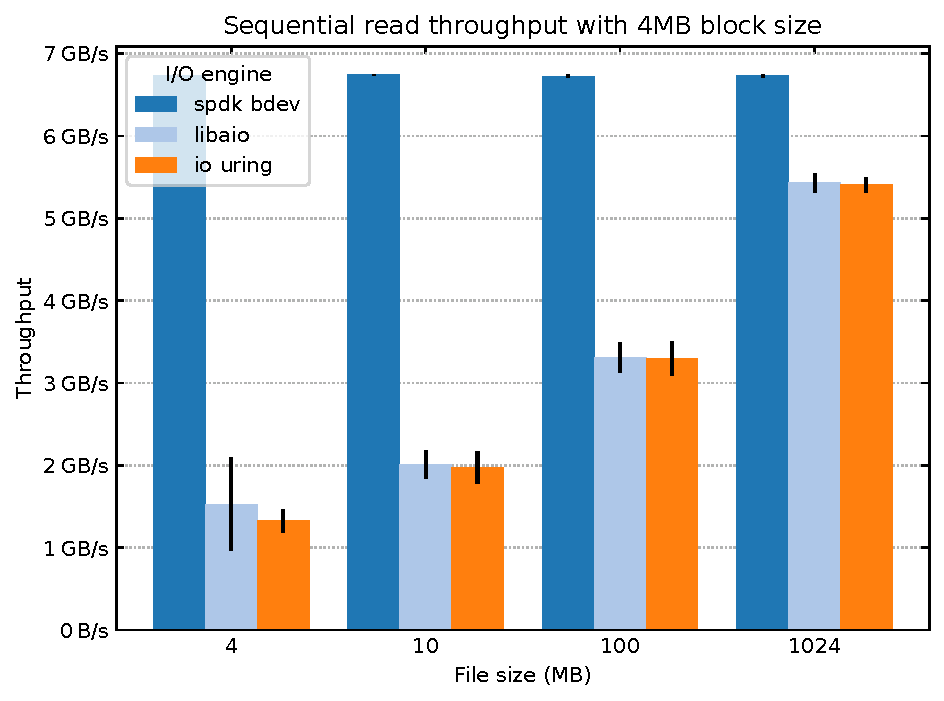
\includegraphics[width=\linewidth]{../measurements/npf/experiments/bs-4M/graphs/read-BANDWIDTH.pdf}
        \caption{Throughput of sequential read operations with 4MB block size}
        \label{fig:read-bandwidth-4M}
    \end{minipage}
    \hfill
    \begin{minipage}{0.48\columnwidth}
        \centering
        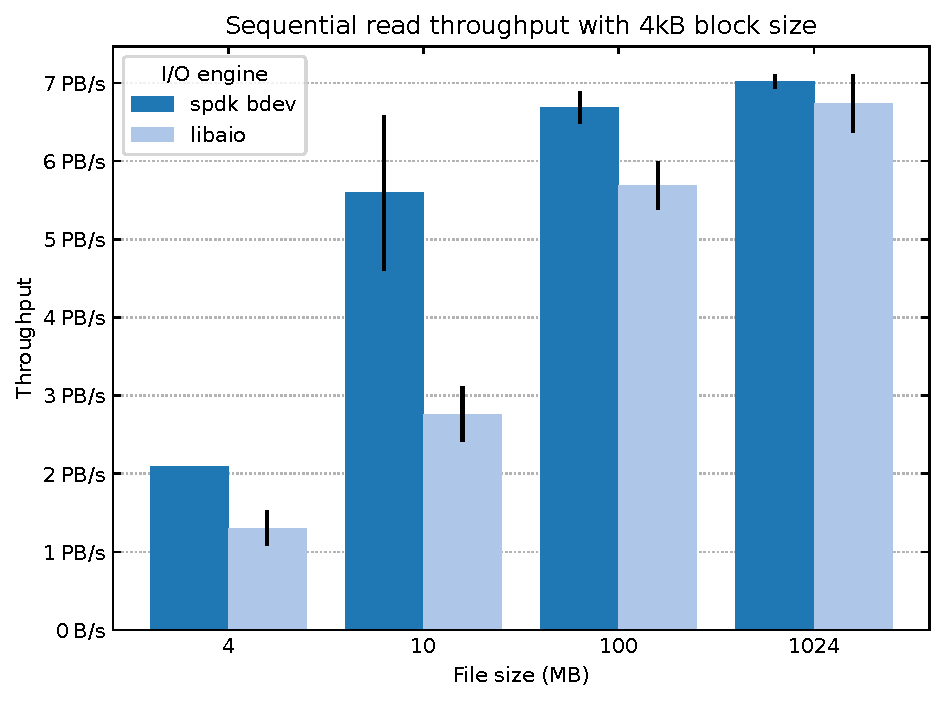
\includegraphics[width=\linewidth]{../measurements/npf/experiments/bs-4K/graphs/read-BANDWIDTH.pdf}
        \caption{Throughput of sequential read operations with 4kB block size}
        \label{fig:read-bandwidth-4K}
    \end{minipage}
\end{figure}

\subsubsection{Sequential write}

For sequential write, the results are less conclusive with 4MB block size. For 4MB and 10MB file size, \acrshort{spdk} performs poorly, being 4 to 5 times slower than Linux kernel. Bigger file size  For 4MB block size, \acrshort{spdk} mean  throughput is 0.3 GB/s while Linux kernel is 1.52 GB/s. For 10MB block size, \acrshort{spdk} throughput is 0.66 GB/s while Linux kernel is 2.58 GB/s. 100MB and 1GB file size on the other side show a significant improvement of \acrshort{spdk} over Linux kernel, with respectively  

\begin{figure}[htbp]
    \centering
    \begin{minipage}{0.48\columnwidth}
        \centering
        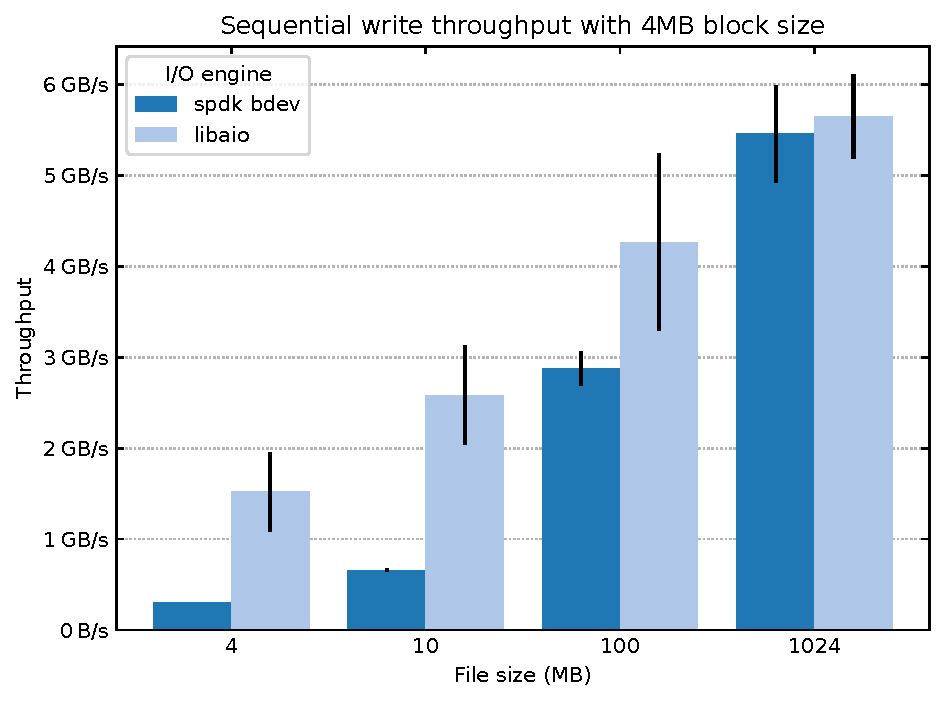
\includegraphics[width=\linewidth]{../measurements/npf/experiments/bs-4M/graphs/write-BANDWIDTH.pdf}
        %\caption{Throughput of sequential write operations with 4MB block size}
        \label{fig:write-bandwidth-4M}
    \end{minipage}
    \hfill
    \begin{minipage}{0.48\columnwidth}
        \centering
        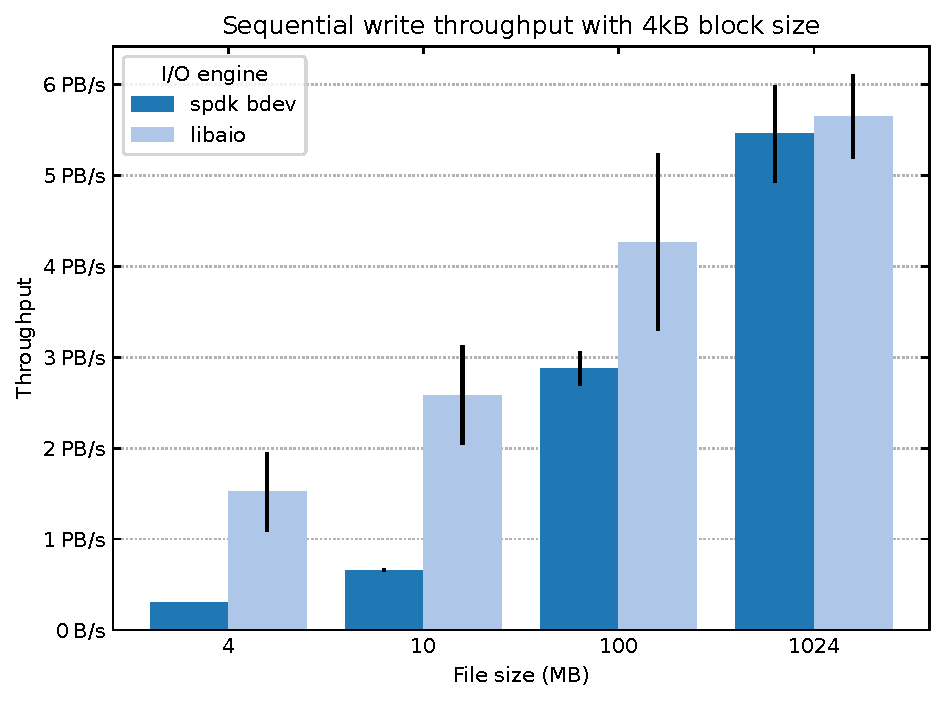
\includegraphics[width=\linewidth]{../measurements/npf/experiments/bs-4K/graphs/write-BANDWIDTH.pdf}
        %\caption{Throughput of sequential write operations with 4kB block size}
        \label{fig:write-bandwidth-4K}
    \end{minipage}
\end{figure}

\subsection{Latency}
    TODO

\section{IO-TCP performances}


\section{Implementation performances}